\section{Paperidra}\label{paperidra}

Tags: Creatura Creatore: Lorenzo CR: 5

\section{Paperidra}\label{paperidra-1}

\begin{center}\rule{0.5\linewidth}{0.5pt}\end{center}

\begin{center}\rule{0.5\linewidth}{0.5pt}\end{center}

\textbf{{[}Monster{]}}

\begin{figure}
\centering
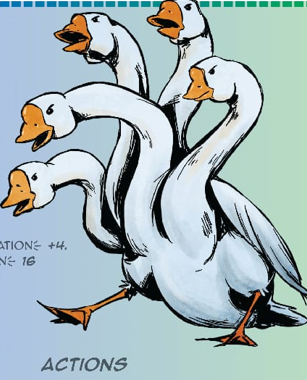
\includegraphics{Screenshot_2023-10-02_154747.png}
\caption{Screenshot 2023-10-02 154747.png}
\end{figure}

Informazioni Generali

Dimensione: Media

Tipo: Demone

Attitude:

Velocità di movimento: 30ft

Habitat: Qualunque

Alleati: Naskirophis, Setta del Sangue

Nemesi: Ordine dei Paladini di San Francesco, Gilda dei Protettori

\begin{center}\rule{0.5\linewidth}{0.5pt}\end{center}

\subsection{1. Descrizione Generale}\label{descrizione-generale}

\begin{center}\rule{0.5\linewidth}{0.5pt}\end{center}

\begin{figure}
\centering
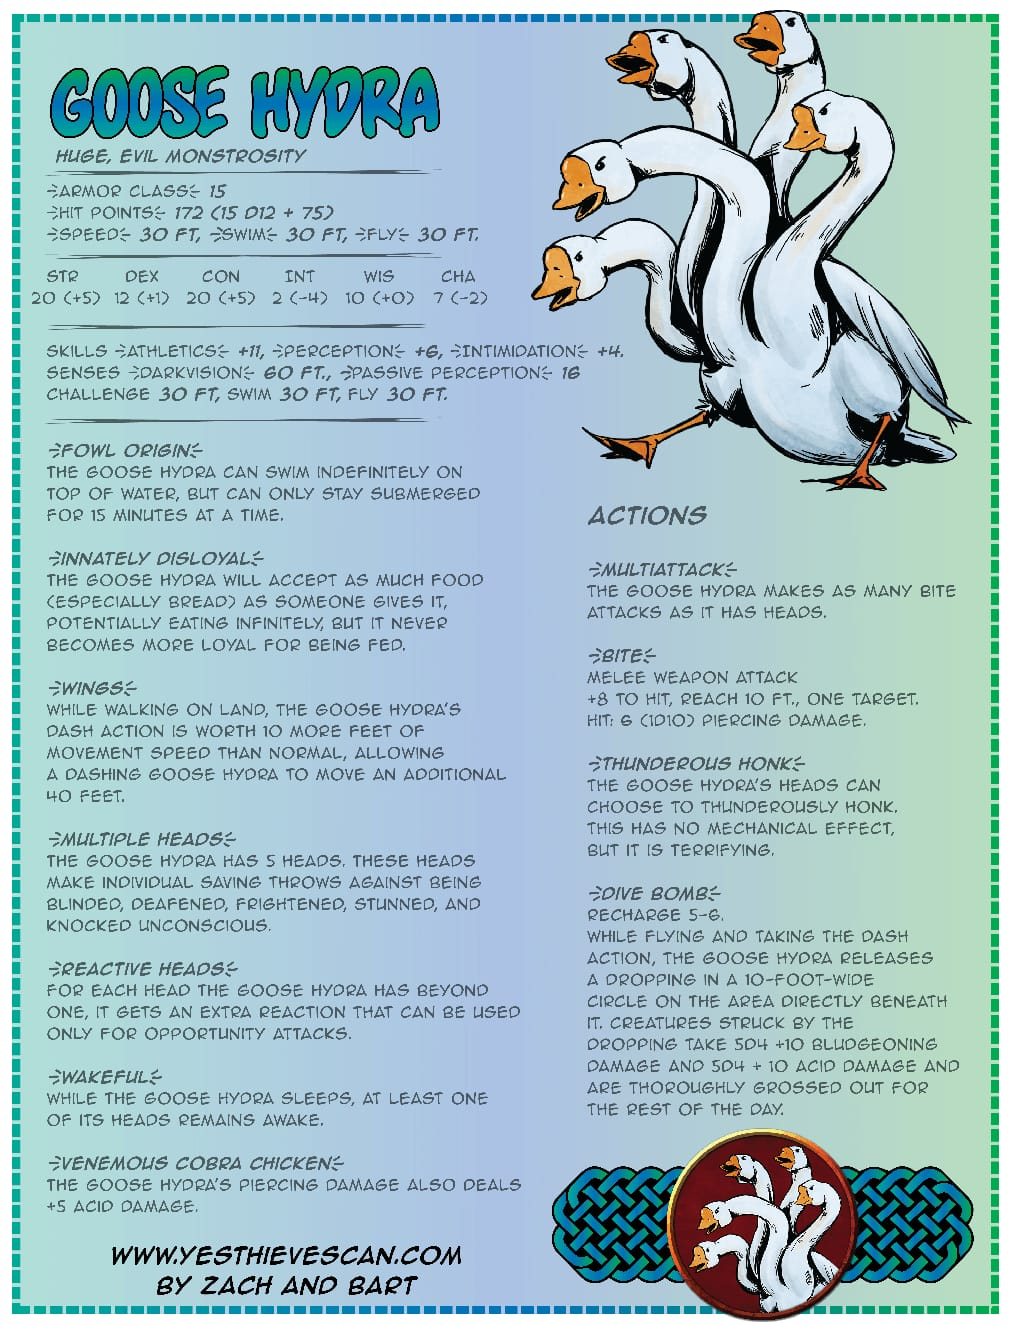
\includegraphics{WhatsApp_Image_2023-10-02_at_15.09.58.jpeg}
\caption{WhatsApp Image 2023-10-02 at 15.09.58.jpeg}
\end{figure}

All'interno delle oscure stanze del Tempio di Naskirophis, un orrore
demoniaco attende coloro che osano minacciare il suo dominio. La Paper
Idra, una creatura mostruosa dai tratti unici e letali, è il prodotto
della fusione di cinque demoni devoti a Naskirophis, membri della
sinistra Setta del Sangue. Questi demoni, dall'aspetto umano ma capaci
di trasformarsi in terribili serpenti con teste di papere, hanno
forgiato un'alleanza oscura per raggiungere un potere senza pari.

Gli accoliti della Setta del Sangue che hanno osato chiedere al loro
signore Naskirophis poteri sovraumani, hanno poi ottenuto la capacità di
trasformarsi in potenti demoni col corpo di serpente e la testa di
anatra. Questi demoni, allo stesso tempo viscidi e piumati, possono
fondersi tra di loro, dando origine alla potente Paperidr

\subsection{2. Distribuzione e Habitat}\label{distribuzione-e-habitat}

\begin{center}\rule{0.5\linewidth}{0.5pt}\end{center}

Qualunque

\subsection{3. Comportamento}\label{comportamento}

\begin{center}\rule{0.5\linewidth}{0.5pt}\end{center}

La Paper Idra è una creatura priva di pietà, sempre pronta a difendere
gli interessi della Setta del Sangue. Ogni testa è capace di muoversi e
agire indipendentemente, ma sono in perfetta sintonia, coordinando i
loro attacchi in un sinistro balletto di morte. La creatura agisce sotto
il controllo delle menti dei demoni che la compongono, e la loro volontà
è irremovibile.

\subsection{4. Variazioni}\label{variazioni}

\begin{center}\rule{0.5\linewidth}{0.5pt}\end{center}

La Paper Idra è il risultato di un rito oscuro che coinvolge la fusione
di cinque demoni della Setta del Sangue. L'unica volta che un esemplare
è stato osservato è stato nel tempio di Naskirophis, durante la missione
\href{Il\%20neonato\%20incasinato\%2090743e94446c4f5a846f18c37fd80698.md}{Il
neonato incasinato}. Non si esclude tuttavia che altri membri della
Setta del Sangue con simili capacità possano dare nuovamente vita ad una
Paperidra, o ad altri mostri demoniaci dal diverso aspetto

\subsection{5. Interazioni con gli
Umani}\label{interazioni-con-gli-umani}

\begin{center}\rule{0.5\linewidth}{0.5pt}\end{center}

Una Paper Idra è stata sconfitta da coraggiosi membri della Gilda dei
Protettori all'interno del Tempio di Naskirophis. Questo incontro fatale
ha portato alla scoperta di questa creatura.
